\documentclass{report}
\usepackage[utf8]{inputenc}
\usepackage[top=0cm, bottom=0cm, left=2cm, right=2cm]{geometry}
\usepackage[francais]{babel}
\usepackage[T1]{fontenc}
\usepackage{graphicx}
\usepackage{subcaption}

\title{Rapport}
\author{François PIAT}
\date{WEEK 1 - 3}

\begin{document}

\maketitle

\chapter*{Contexte}

\paragraph{L'environnement de travail:}
Dans le cadre de ma 4\up{ème} année à l'INSA Centre Val de Loire, j'ai effectué un stage de 18 semaines dans le laboratoire BioMedIA, implanté sur le campus de l'Imperial College à Londres. Ce laboratoire dévoloppe les outils informatiques nécessaires à des chercheurs en milieu médical, et majoritairement en neurologie. 

\paragraph{Le sujet du stage:} Le sujet du stage proposé est le suivant:
\textit{ \begin{quote}
Développement d'une bibliothèque mathématique performante pour le traitement d'images
médicales
\end{quote} } 
Le stage consiste à optimiser un logiciel de traitement d'images nommé MIRTK (Medical Image Registration ToolKit), codé en C++. L'action principale s'effectuera sur le module "Numerics" du logiciel, qui fait, entre autres, le lien entre une bibliothèque mathématique (nommée EIGEN) et MIRTK.\newline Le principe majeur du stage consiste à adapter une autre bibliothèque mathématique nommée ArrayFire pour plusieurs raisons explicitées dans la suite du rapport.
\newline\newline \begin{center}{L'architecture du logiciel est détaillée ci-dessous:} \end{center}

\begin{figure}[h!]
	\begin{center}
	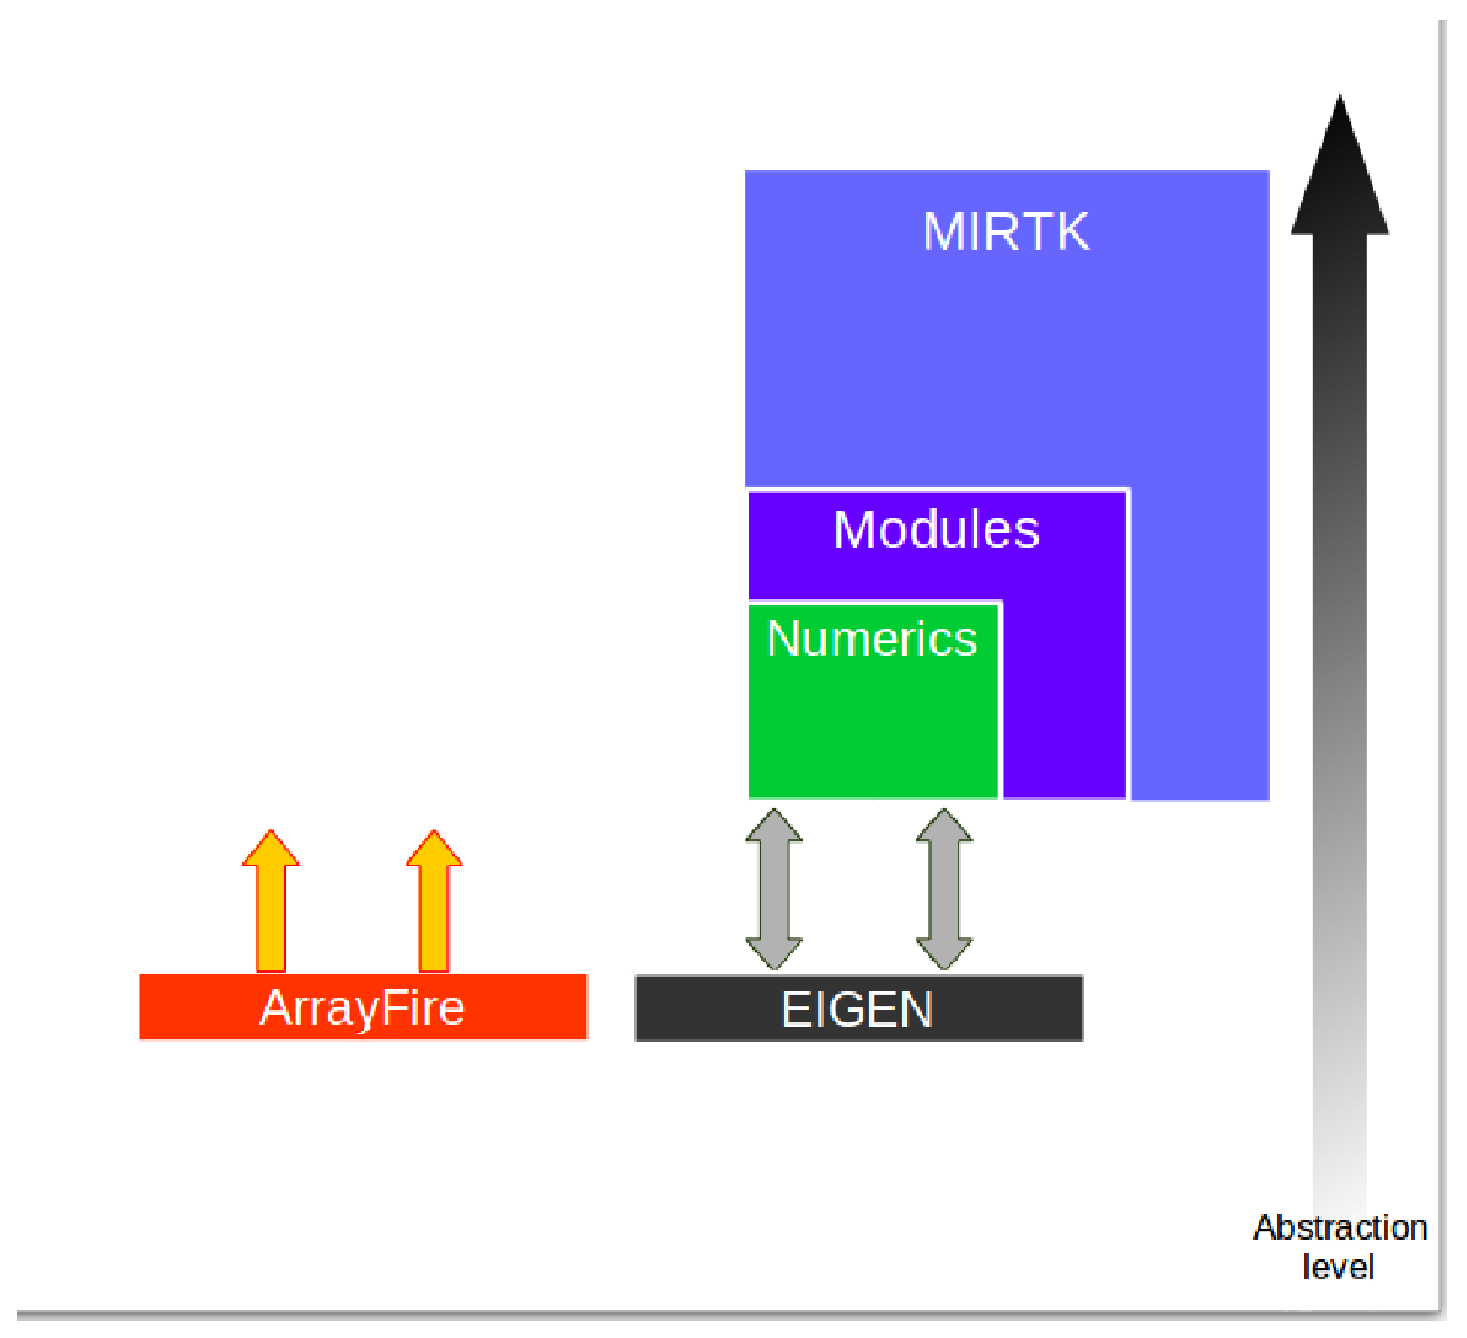
\includegraphics[height=8cm]{figures/struc.eps}
	\end{center}	
	\caption{Structure logicielle}
	\label{Structure logicielle}
\end{figure}

\chapter*{Etude de MIRTK et EIGEN}

\paragraph{Dépendance:} 

Le module Numerics emprunte plusieurs fonctions issues de la bibliothèque EIGEN. Cette dépendance est décrite par le diagramme suivant: 

\begin{figure}[h!]
	\begin{center}
		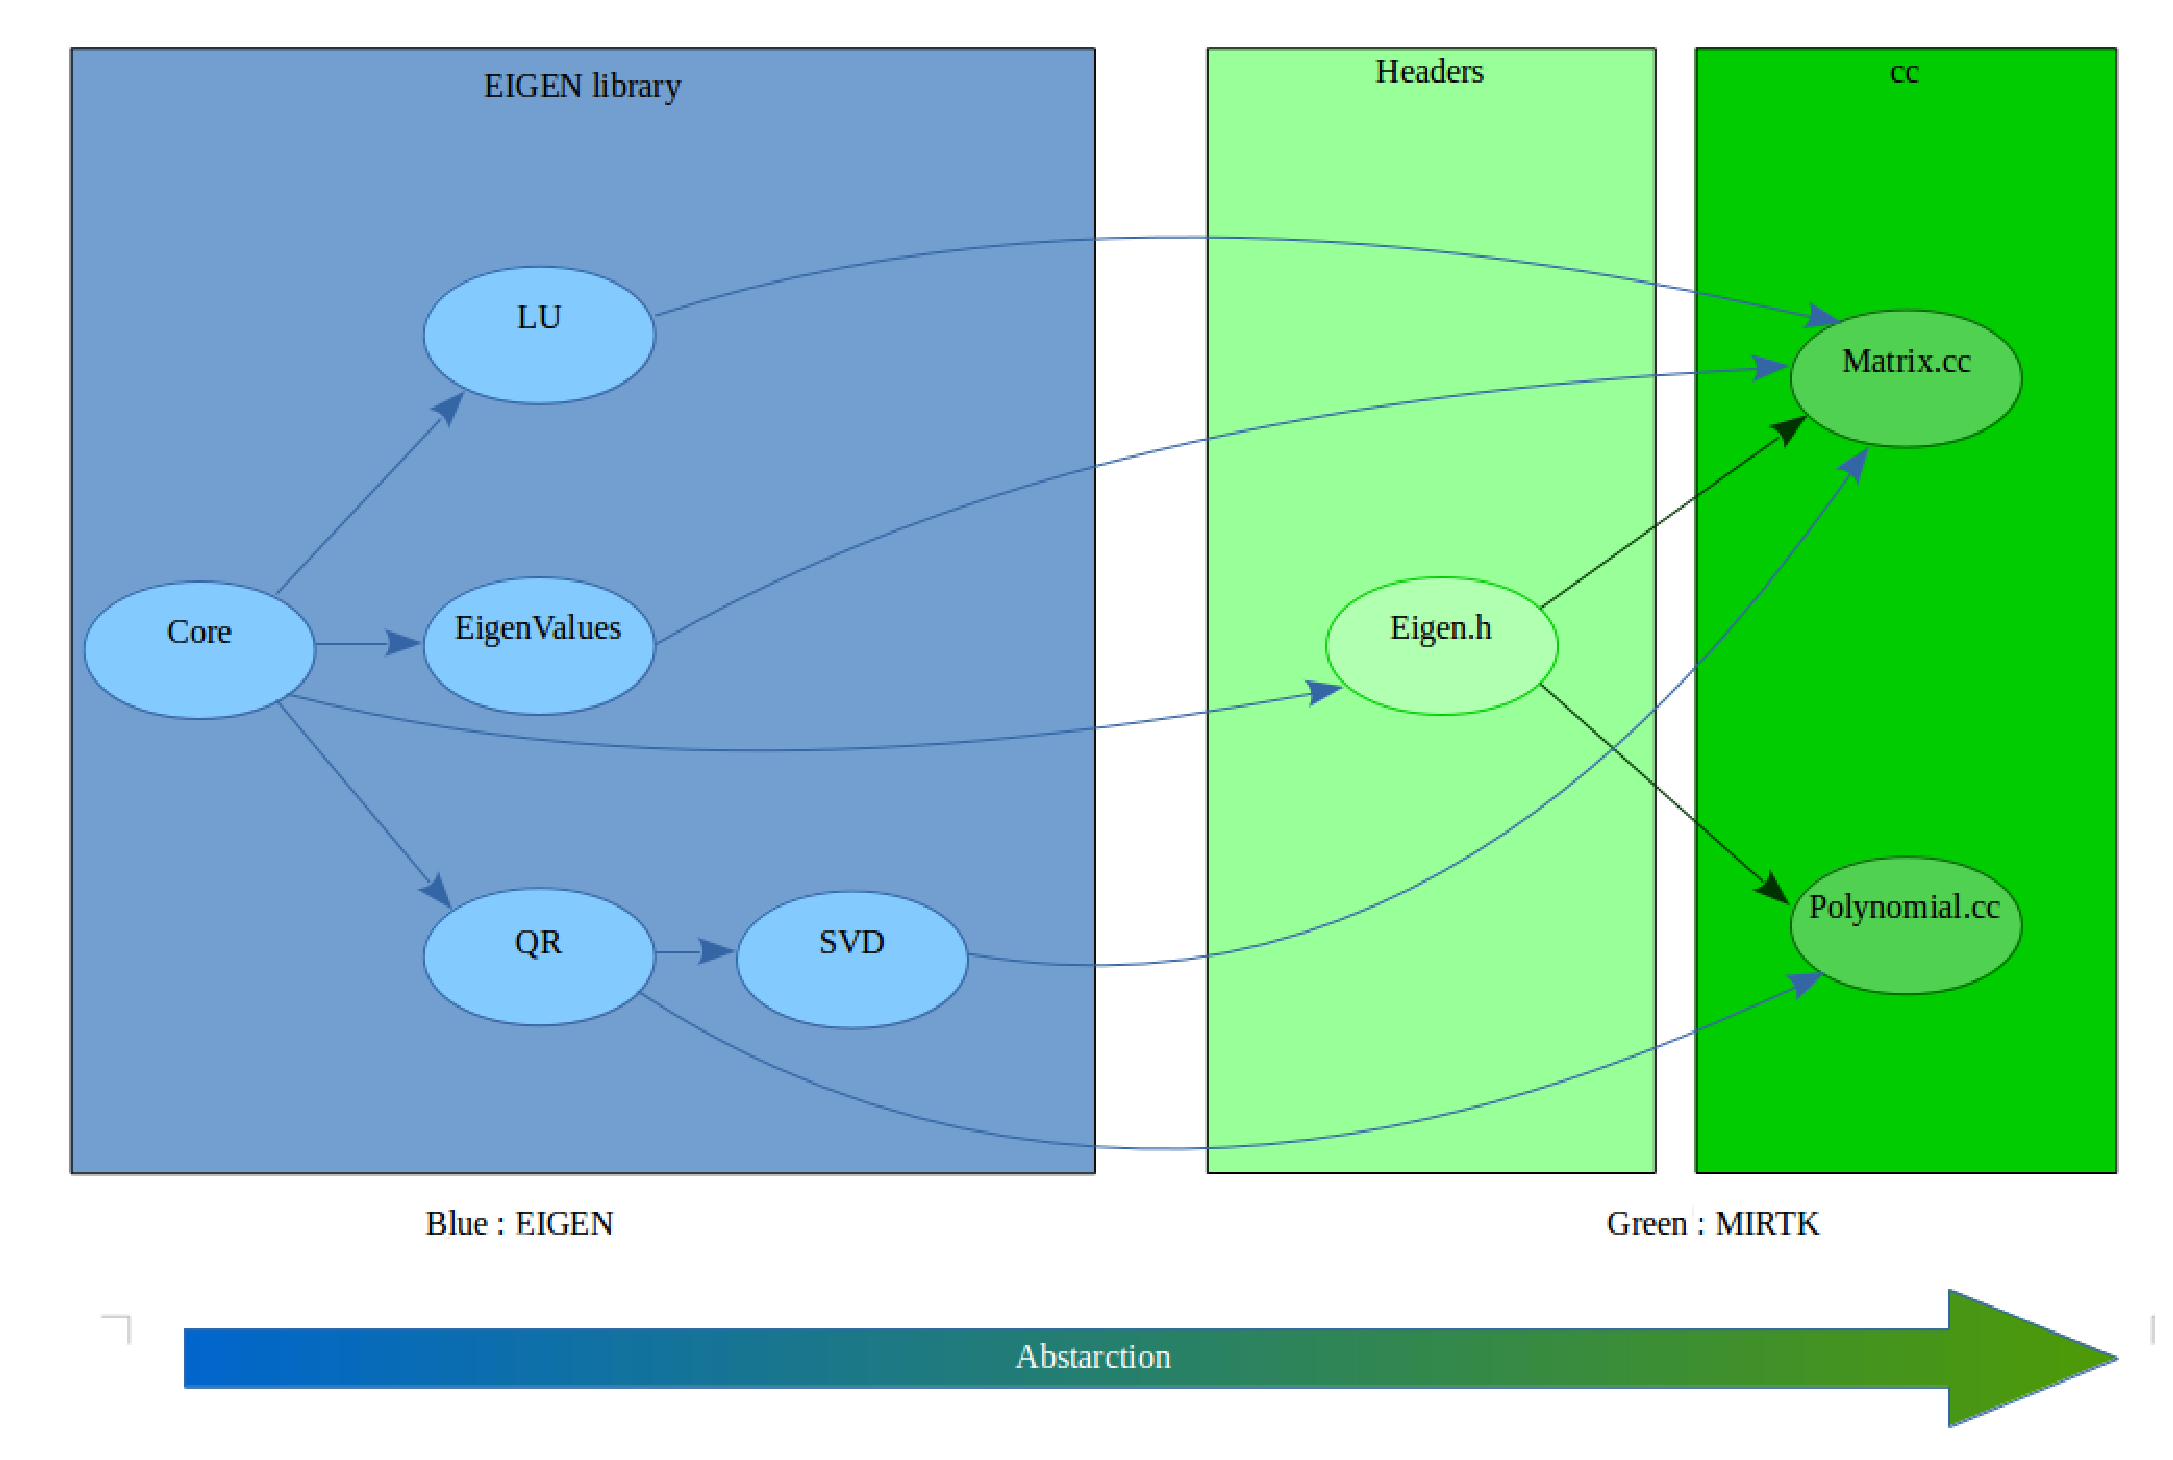
\includegraphics[width=16cm]{figures/eigen_mirtk.eps}
	\end{center}	
	\caption{Dépendance MIRTK/EIGEN}
	\label{Dépendance MIRTK/EIGEN}
\end{figure}

Chaque bulle représente un fichier, soit source (contenant donc l'implémentation des fonctions), soit header. La signification d'une flèche est "...est appelé dans...". Ainsi, par exemple, LU est appelé dans Matrix.cc. 

\paragraph{Problème:}
 Le fichier "Eigen.h" est en fait un fichier intermédiaire qui convertit des vecteurs/matrices issus de la bibliothèque Eigen en vecteurs/matrices utilisés dans MIRTK, et vice-versa.
 
\textit{\t Solution: } Créer un fichier de façade, qui agisse de la même manière avec une adaptation pour ArrayFire

\chapter*{Etude d'ArrayFire}

\paragraph{L'API:}
Cette étude a pour but de cerner les fonctions et classes qui vont intervenir dans le module Numerics, et qui remplaceront la structure basée sur Eigen. Beaucoup de fonctions utilisées par Eigen, telles que la SVD (Singular Values Decomposition), ou la LU (Lower Upper Decomposition) sont implémentées dans ArrayFire et pourront remplacer les fonctions appelées dans MIRTK de manière quasiment similaire. Ces fonctions agissent principalement sur des matrices et/ou des vecteurs.

En revanche, tout le design des tableaux ainsi que plusieurs méthodes sont propres à ArrayFire et nécessiteront des modifications du code de MIRTK pour ne pas modifier l'exécution de celui-ci (qui doit rester la même!).

\paragraph{La programmation parallèle:}
La programmation parallèle est une partie de l'implémentation et du design d'un projet qui lui permet de fonctionner en utilisant davantage de ressources sur une machine, optimisant donc les performances. Ce projet va surtout s'intéresser à l'optimisation des itérations, majoritairement au sein de boucles \textit{"for"}.
La fonction d'ArrayFire qui va permettre cette programmation parallèle s'appelle \textit{"gfor"} et fonctionne de la manière suivante :

\begin{figure}[h!]
	\begin{center}
		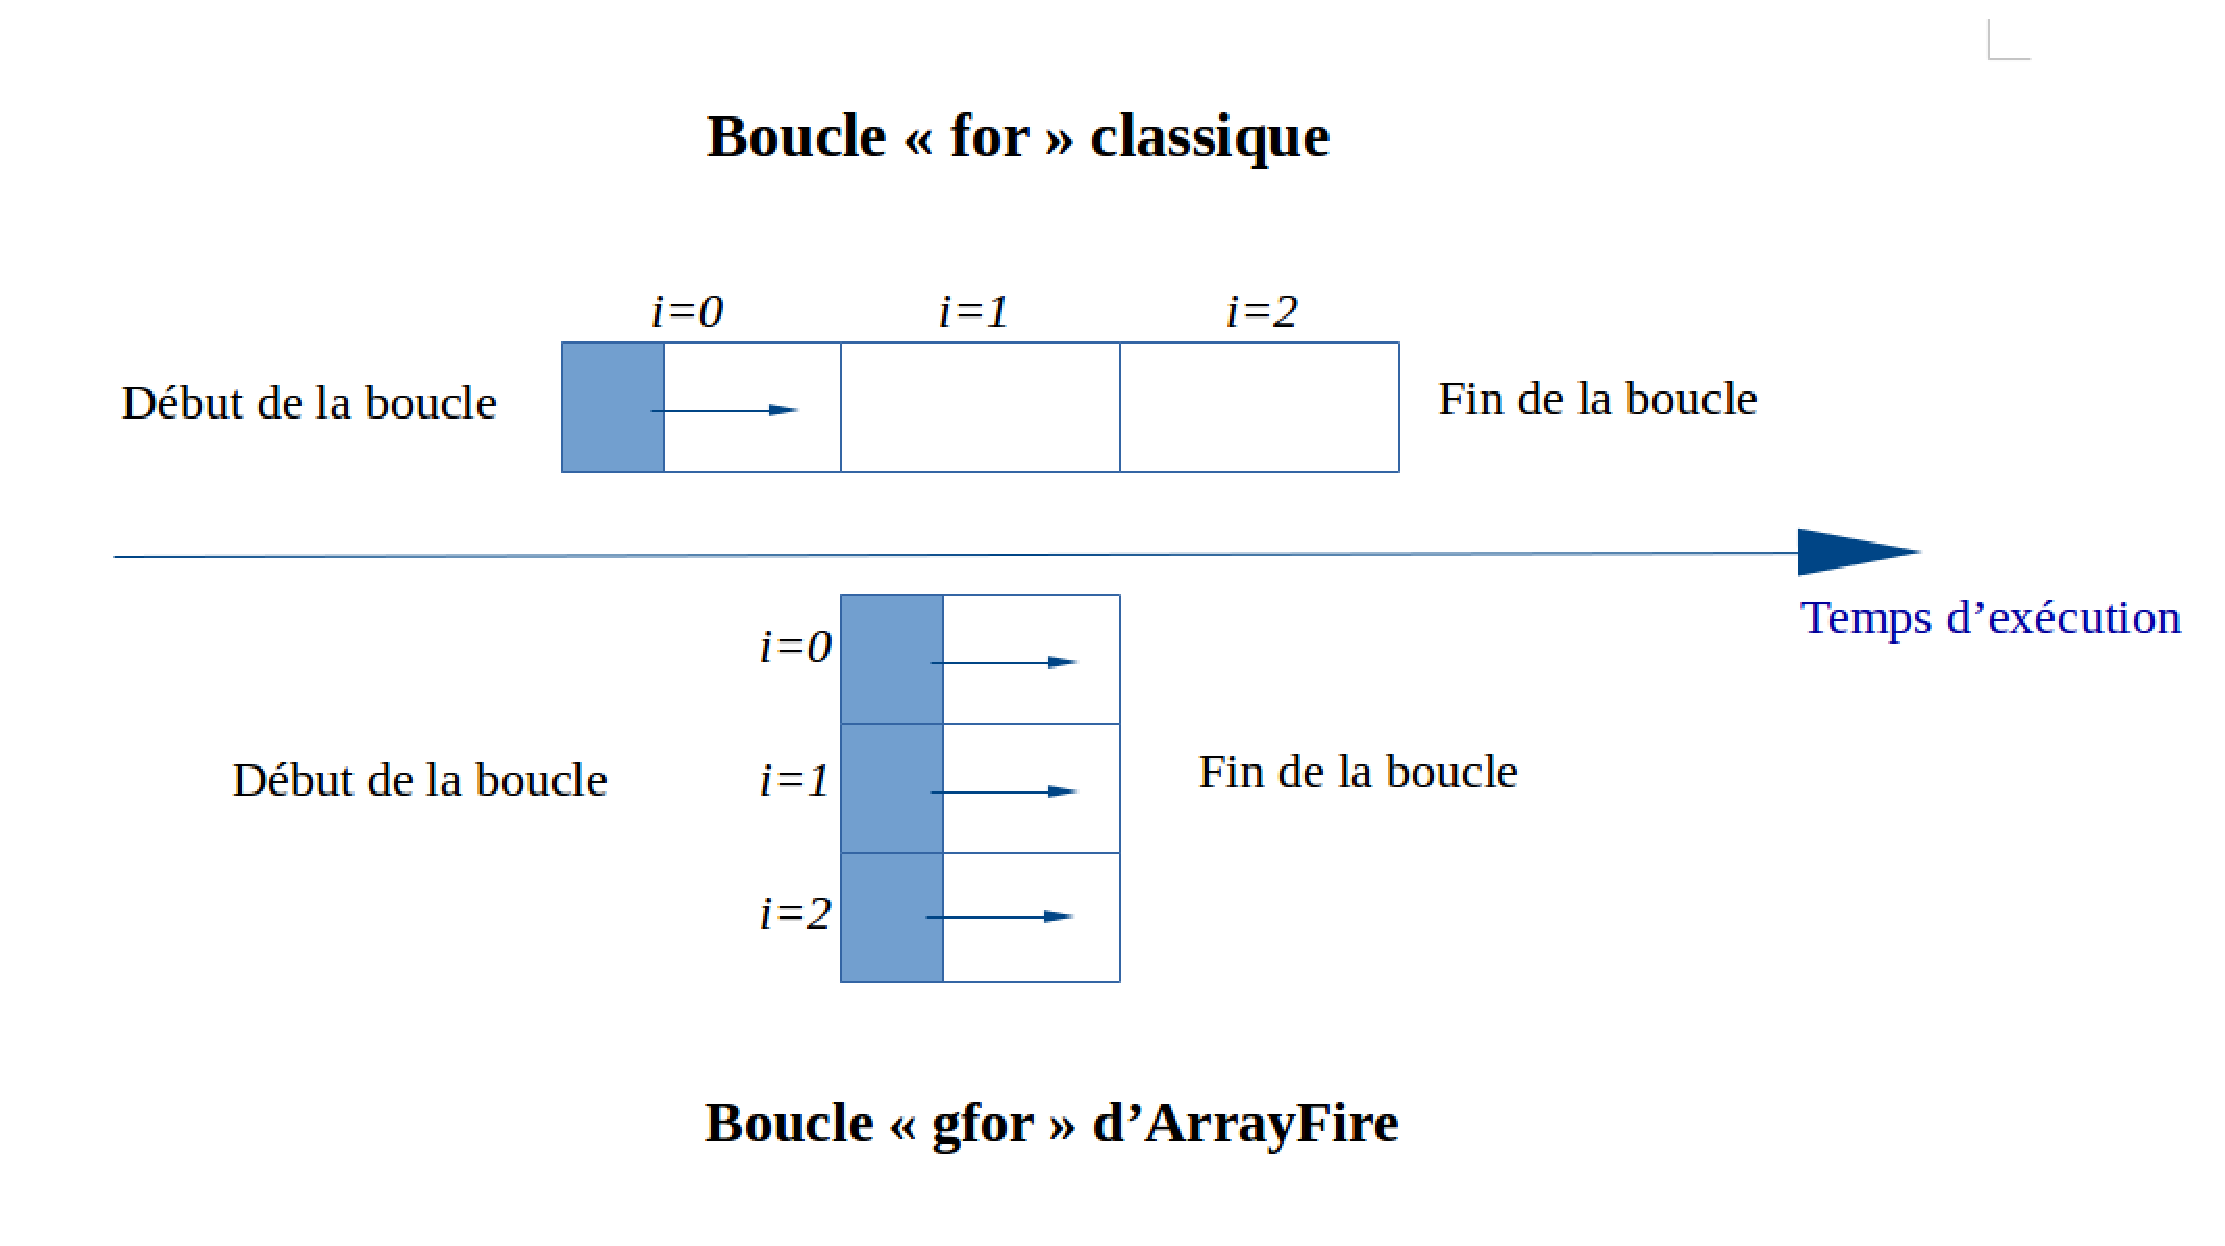
\includegraphics[width=14cm]{figures/gfor.eps}
	\end{center}	
	\caption{Fonctionnement de gfor}
	\label{Fonctionnement de gfor}
\end{figure}

Au lieu d'itérer une variable de manière temporelle, la fonction \textit{"gfor"} va déclarer plusieurs \textit{threads}, qui sont différents canaux d'exécution. Sur la FIGURE 3 ci-dessus, un thread est représenté par un rectangle. Ainsi, pour une boucle classique, le même thread est utilisé plusieurs fois consécutivement. 

La syntaxe de gfor indique qu'il n'y a pas d'itérateur. C'est bel et bien un tableau qui va être déclaré, ayant dans chaque case la valeur souhaitée. Par exemple, dans la FIGURE 3 ci-dessus, le tableau de valeur "i" serait la séquence suivante: [0,1,2].

\chapter*{Etude de TBB dans MIRTK}
\paragraph{La programmation parallèle:}
\textit{Threading Building Blocks} (abrégé TBB) est une bibliothèque fournie par Intel, et qui permet la gestion de threads dans du code C++. Cette bibliothèque est utilisée par MIRTK et l'idéal serait de le remplacer, dans la limite du possible, par la fonction "gfor", issue d'ArrayFire et précédemment explicitée.
La syntaxe de TBB étant particulièrement lourde, l'arrivée d'ArrayFire pourra "alléger" le code.
\newline\newline
Syntaxe TBB / Syntaxe gfor ici...
\newline\newline
Listing établi de toutes les utilisations de blocked-range dans le code de MIRTK, puis classification en fonction du parttern utilisé à chaque fois.

\chapter*{Bazar}
- Pour une bonne optimisation, il faut toujours agir sur les opérations les plus atomiques. Si une parrallélisation se fait sur un code entier, comprenant des conditions (if, while...), il faudra toujours attendre que le dernier thread ait fini son opération pour avancer (+ interventions extérieur nécessitant ce thread, comme des requetes http, des notifications...)

- L'image est un ensemble de pixels. Chaque pixel définit sa couleur par la combinaison de 3 LEDs. Cette combinaison de couleurs est modélisée pour MIRTK sous forme de vecteurs. Chaque vecteur représente le sens d'évolution de l'image: 

\begin{figure}[h!]
	\begin{center}
		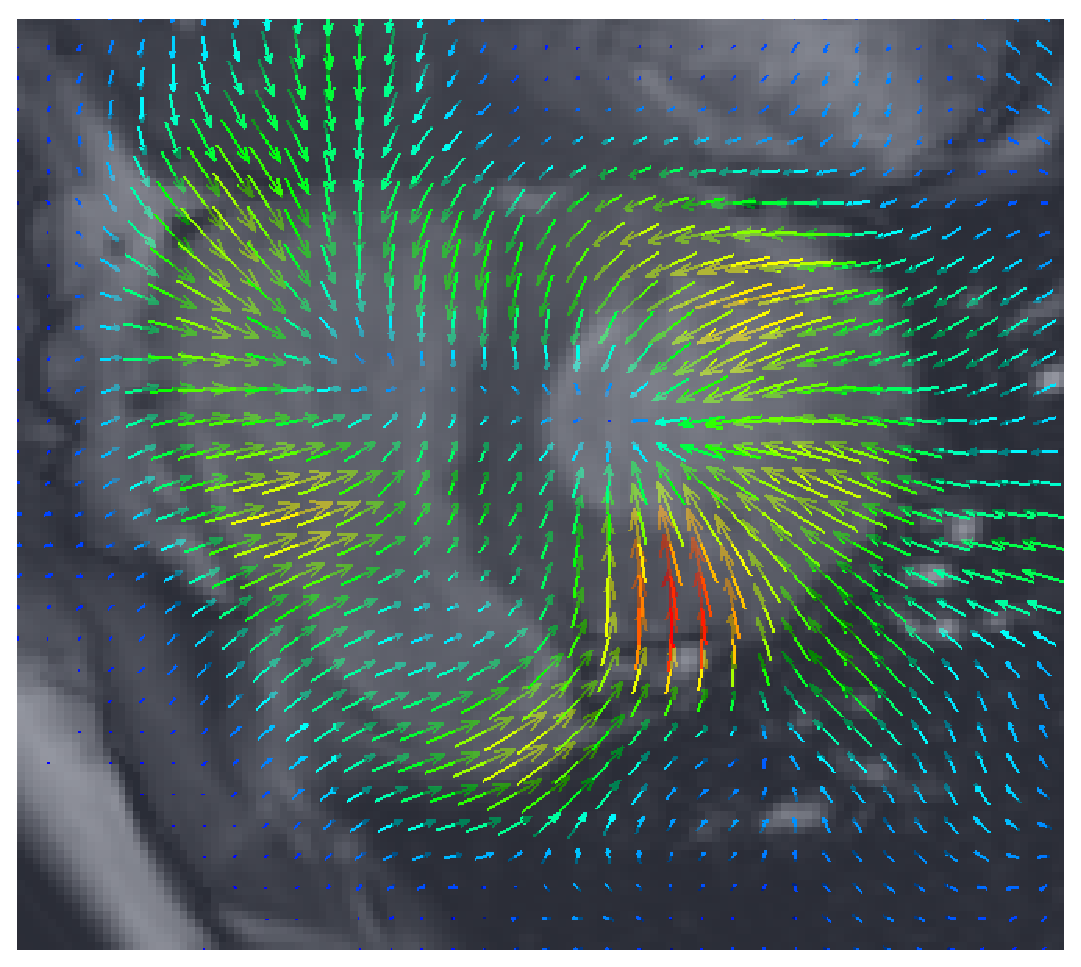
\includegraphics[width=8cm]{figures/field.eps}
	\end{center}	
	\caption{Fonctionnement de gfor - \textit{www.inria.fr}}
	\label{Fonctionnement de gfor}
\end{figure}

- Profiling = ? , nécessaire? profiling= méthode de détection des fonctions et des commandes qui utilisent le plus de ressources et le plus de temps sur la machine lorsque le code s'éxécute.


% Exemple de double figure

%\begin{figure}[h]
%	
%	\begin{subfigure}{0.5\textwidth}
%		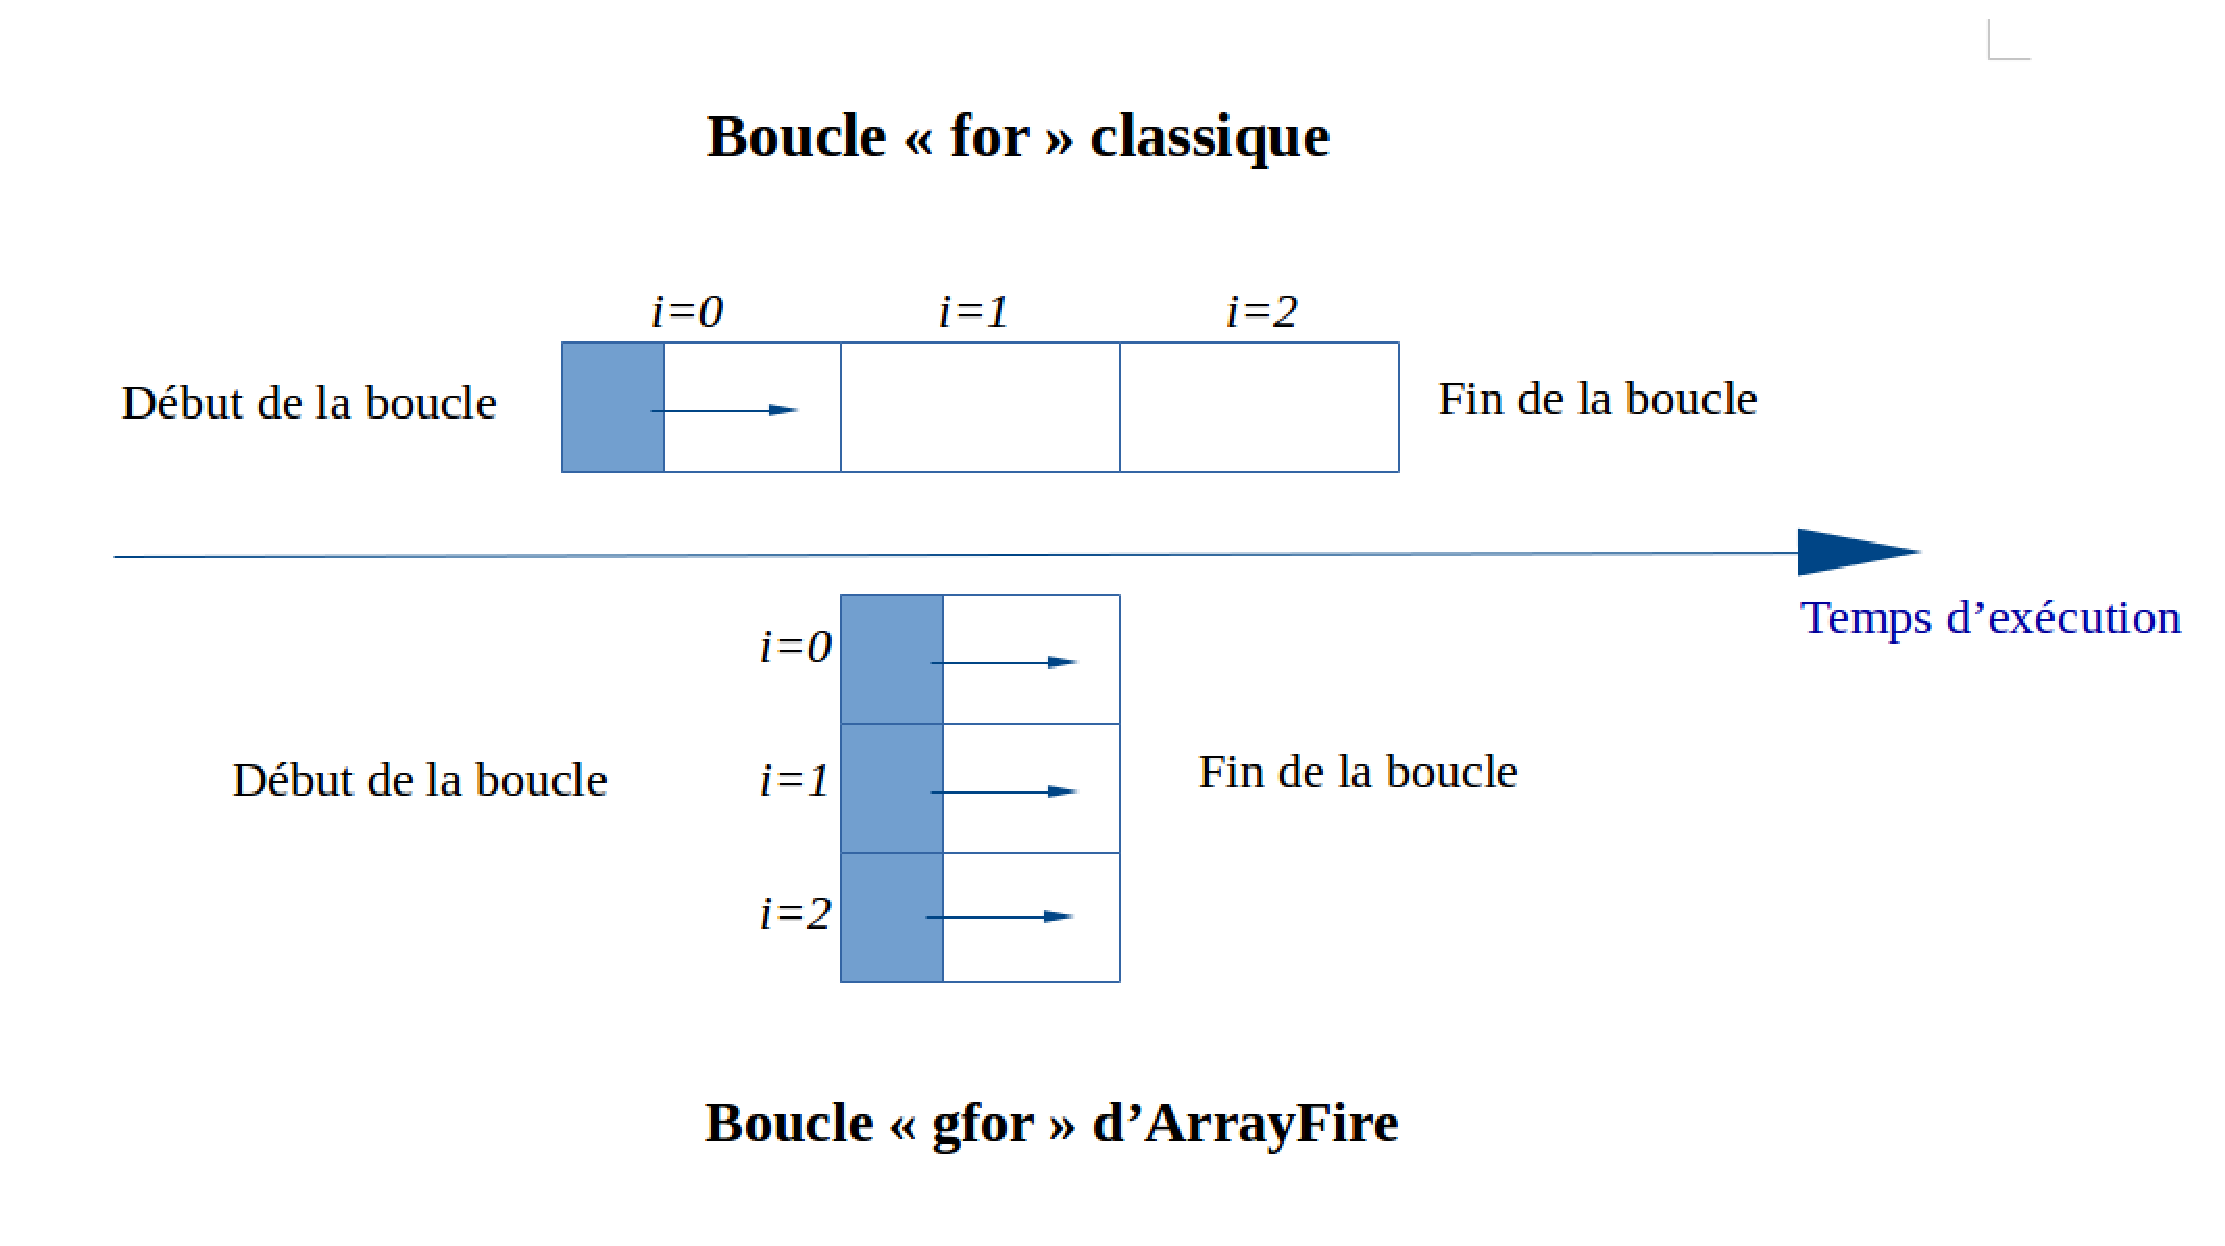
\includegraphics[width=0.9\linewidth, height=5cm]{figures/gfor.eps} 
%		\caption{Caption1}
%		\label{fig:subim1}
%	\end{subfigure}
%	\begin{subfigure}{0.5\textwidth}
%		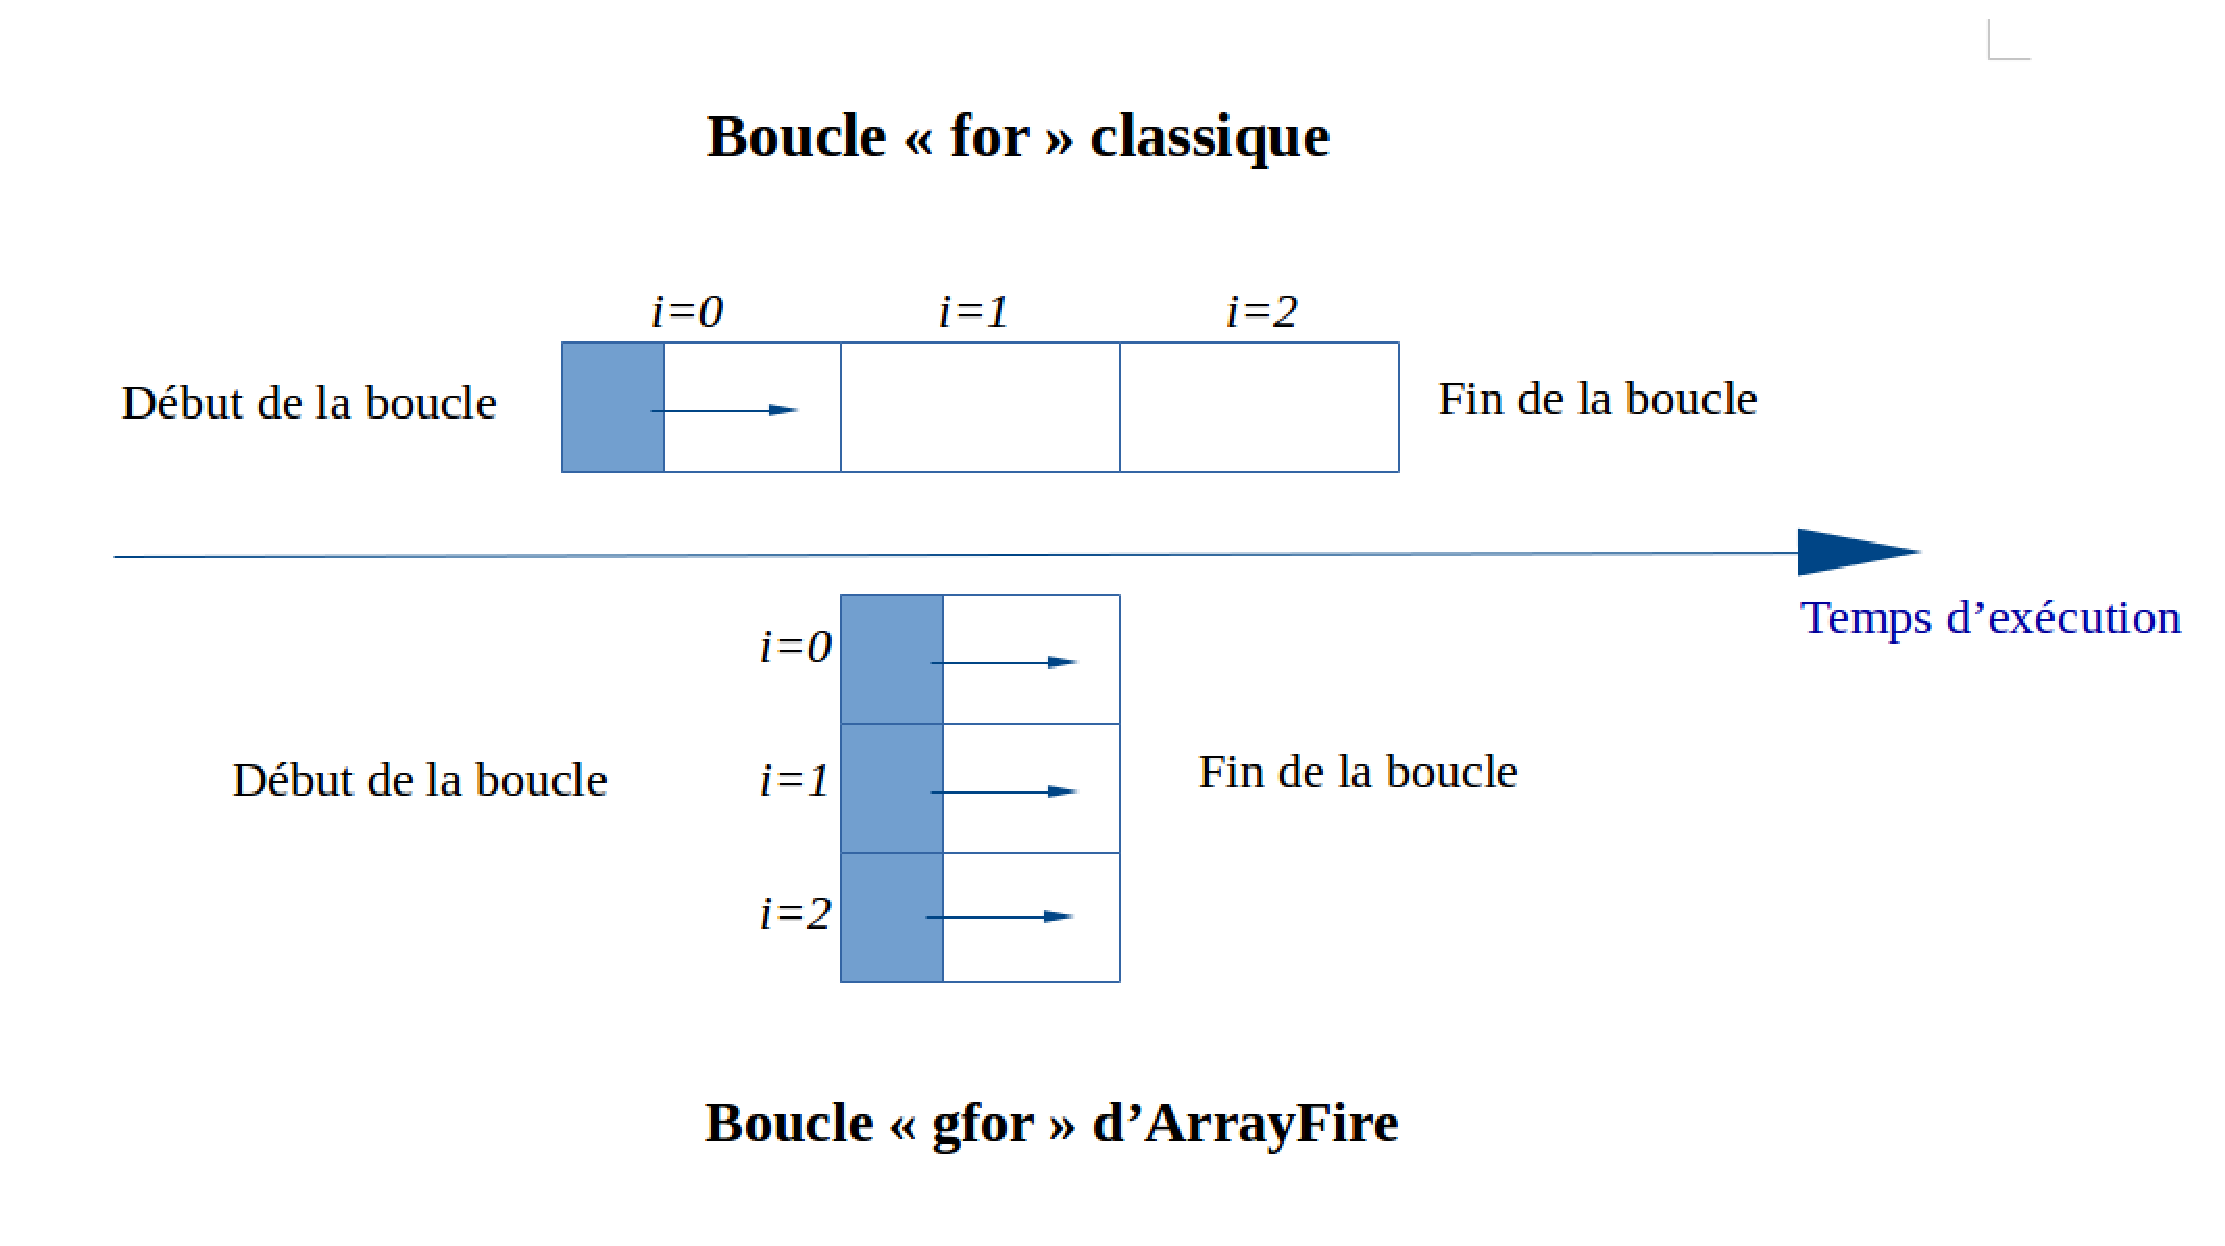
\includegraphics[width=0.9\linewidth, height=5cm]{figures/gfor.eps}
%		\caption{Caption 2}
%		\label{fig:subim2}
%	\end{subfigure}
%	
%	\caption{Caption for this figure with two images}
%	\label{fig:image2}
%\end{figure}

\end{document}
